\chapter{Week 1}
\section{What is a time series?}
\usemintedstyle{pastie}
In classical statistics, we normally consider $ X_1,\ldots,X_n\in\mathbf{R}^p $,
a \textbf{simple random sample}.

In particular,
\begin{enumerate}[(1)]
    \item $ X_1,\ldots,X_n $ are i.i.d. (independent and identically distributed)
    \item $ X_i \sim F_\theta $ which is a common distribution characterized
          by $ \theta $.
\end{enumerate}
Examples:
\begin{enumerate}
    \item $ X_i \stackrel{\text{iid}}{\sim} \N{\mu,\sigma^2} $, and we wish to estimate
          and perform inference on $ \mu $ and $ \sigma^2 $.
    \item $ X_i=\begin{bmatrix}
                  Y_i \\
                  Z_i
              \end{bmatrix} $ where $ Y_i $ is a dependent variable, and
          $ Z_i $ is an independent variable.
              {\color{blue}Perhaps we happen to observe
                  $ Y_i $ and $ Z_i $ in pairs, and we posit a model:}
          \[ Y_i=\beta^\top Z_i+\varepsilon_i,\quad\varepsilon_i
              \stackrel{\text{iid}}{\sim} \N{0,\sigma_{\varepsilon}^2} \]
          \begin{Remark}{}{}
              The relationship between $ Y_i $ and $ Z_i $ doesn't
              depend on $ i $, it only depends upon the common parameter
              $ \beta $, and it assumes that $ \varepsilon_i $ has fixed variance
              for each $ i $.
          \end{Remark}
    \item In such settings, one is typically interested in:
          \begin{enumerate}
              \item Prediction: {\color{blue} based on the data, how can we predict
                    the behaviour of these variables in the future?}
              \item Inference: {\color{blue}how do we use the data to try to estimate
                    and better understand the underlying mechanism which generates
                    the data? For example, a linear model or simple Gaussian model.}
          \end{enumerate}
\end{enumerate}
\begin{Definition}{Time series}{}
    We say $ X_1,\ldots,X_T $ is an (observed)
    \textbf{time series} of length $ T $ if $ X_t $
    denotes an observation obtained at time $ t $.
    In particular, the observations are ordered in time.
\end{Definition}
\begin{Definition}{Real-valued time series}{}
    If $ X_t\in\mathbf{R} $, we say $ X_1,\ldots,X_T $ is
    a \textbf{real-valued} (\textbf{scalar}) \textbf{time series}.
\end{Definition}
\begin{Definition}{Multivariate time series}{}
    If $ X_t\in\mathbf{R}^p $, we say $ X_1,\ldots,X_T $
    is a \textbf{multivariate} (\textbf{vector-valued})
    \textbf{time series}.
\end{Definition}

\begin{figure}[!htbp]
    \centering
    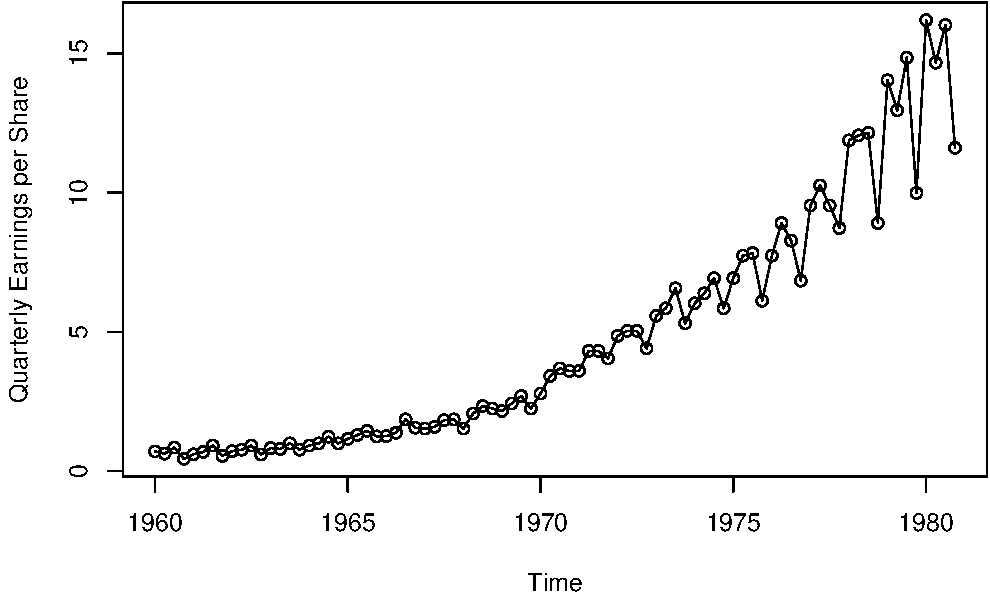
\includegraphics[width=0.75\textwidth]{jj.pdf}
    \caption{Quarterly Johnson and Johnson Earnings}\label{fig:jj}
\end{figure}
\begin{minted}{R}
# Figure 1.1
plot(jj, type = "o", ylab = "Quarterly Earnings per Share")
\end{minted}
Observe that in~\Cref{fig:jj}:
\begin{itemize}
    \item The earnings are steadily increasing over time.
    \item There is heterogeneity in the variance over time.
\end{itemize}

With time series data, we are typically concerned
with the same goals as in classical statistics (prediction and inference).
However, in contrast with time series, the data often exhibit:
\begin{enumerate}[(1)]
    \item \textbf{Heterogeneity}
          \begin{itemize}
              \item Time trends $ \rightarrow \E{X_t}\neq \E{X_{t+h}} $.
              \item Heteroskedasticity
                    $ \rightarrow \Var{X_t}\neq \Var{X_{t+h}} $.
          \end{itemize}
          {\color{blue}In classical statistics, it's assumed that all the observations have the
          same distribution which is clearly \underline{not} the case in time series.}
    \item \textbf{Serial Dependence (Serial Correlation)}
          \begin{itemize}
              \item Observations that are temporally close appear to depend
                    on each other.
          \end{itemize}
          {\color{blue}In classical statistics, each successive observation is assumed
          to be independent which is clearly \underline{not} the case in time series.}
\end{enumerate}

\begin{figure}[!htbp]
    \centering
    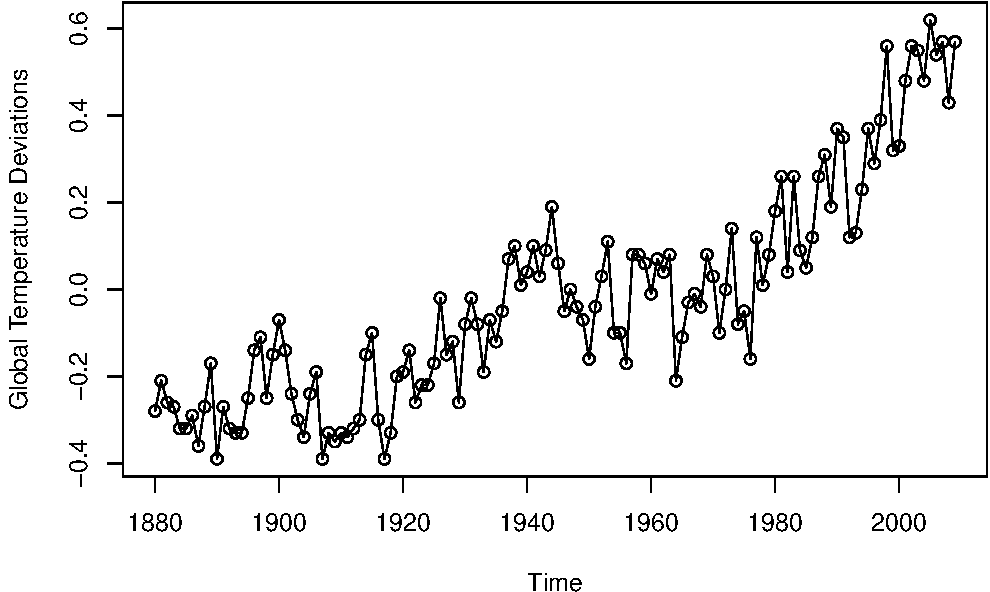
\includegraphics[width=0.75\textwidth]{gtemp.pdf}
    \caption{$ x_t $ is the deviation of global mean
        yearly temperature from the mean computed from 1951 to 1980}\label{fig:gtemp}
\end{figure}
\begin{minted}{R}
# Figure 1.2
plot(gtemp, type = "o", ylab = "Global Temperature Deviations")
\end{minted}
Observe that in~\Cref{fig:gtemp}:
\begin{itemize}
    \item The global temperature is steadily increasing over time.
    \item Heterogeneity exists within the mean over time.
    \item Heterogeneity exists within the variance over time, although it is not very apparent.
    \item Serial dependence occurs.
\end{itemize}
Let's formally define a time series.
\begin{Definition}{Time series, Observed stretch}{}
    We say $ \set{X_t}_{t\in\mathbf{Z}} $
    is a \textbf{time series} if $ \set{X_t : t\in\mathbf{Z}} $
    is a stochastic process indexed by $ \mathbf{Z} $.
    In other words, there is a common probability space
    $ (\Omega,\mathcal{F},\mathbb{P}) $ such that
    $ X_t:\Omega\to\mathbf{R} $ is a random variable
    for all $ t $.

    In relation to the original definition, we say
    $ X_1,\ldots,X_T $ is an \textbf{observed stretch} (\textbf{realization},
    \textbf{simple path}) of length $ T $ from $ \set{X_t}_{t\in\mathbf{Z}} $.
\end{Definition}
{\color{blue}Formally speaking, we think of a time series as being a little snippet
of one long sample path the stochastic process for which would characterize
all the serial dependence, time trends, and heteroskedasticity
that exist within a time series as can be seen in~\ref{fig:1.1_f1}.}
\begin{figure}[!htbp]
    \centering
    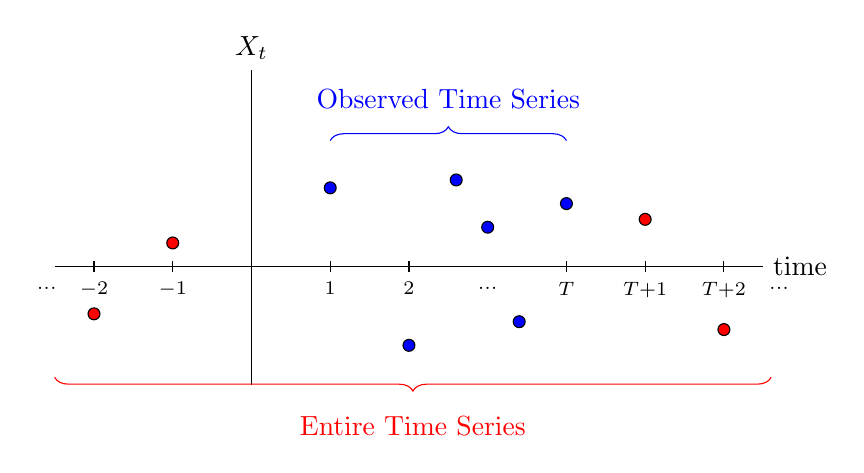
\begin{tikzpicture}
        \draw (-2.5,0) -- (6.5,0) node[right] {time};
        \draw (0,-1.5) -- (0,2.5) node[above] {$X_t$};

        \foreach \x/\xtext in {-2/-2, -1/-1, 1/1, 2/2, 4/T, 5/T+1, 6/T+2}
        \draw[shift={(\x,0)}] (0pt,2pt) -- (0pt,-2pt) node[below] {$\scriptstyle\xtext$};

        \draw (-2.6,0) node[below,yshift=-4pt] {$\scriptstyle\ldots$};
        \draw (3,0) node[below,yshift=-4pt] {$\scriptstyle\ldots$};
        \draw (6.7,0) node[below,yshift=-4pt] {$\scriptstyle\ldots$};

        \draw[fill=red] (-2,-.6) circle (.5ex);
        \draw[fill=red] (-1,0.3) circle (.5ex);
        \draw[fill=blue] (1,1) circle (.5ex);
        \draw[fill=blue] (2,-1) circle (.5ex);
        \draw[fill=blue] (2.6,1.1) circle (.5ex);
        \draw[fill=blue] (3,0.5) circle (.5ex);
        \draw[fill=blue] (3.4,-.7) circle (.5ex);
        \draw[fill=blue] (4,.8) circle (.5ex);
        \draw[fill=red] (5,.6) circle (.5ex);
        \draw[fill=red] (6,-.8) circle (.5ex);

        \draw [decorate,decoration={brace,amplitude=5pt,mirror,raise=4ex},color=red]
        (-2.5,-0.8) -- (6.6,-0.8) node[midway,yshift=-3.5em,text=red]{Entire Time Series};
        \draw [decorate,decoration={brace,amplitude=5pt},color=blue]
        (1,1.6) -- (4,1.6) node[midway,yshift=1.5em,text=blue]{Observed Time Series};
    \end{tikzpicture}
    \caption{Time Series}\label{fig:1.1_f1}
\end{figure}
\section{Basic Principles of Forecasting}
Consider a time series of length $ T $, namely $ X_1,\ldots,X_T $.
Based on $ X_1,\ldots,X_T $, we would like to produce a ``best guess''
for $ X_{T+h} $:
\[ \hat{X}_{T+h}=\hat{X}_{T+h\mid T}=f_h(X_T,\ldots,X_1) \]
\begin{Definition}{Forecast, Horizon}{}
    For $ h\ge 1 $, our ``best guess''
    \[ \hat{X}_{T+h}=f_h(X_T,\ldots,X_1) \]
    is called a \textbf{forecast} of $ X_{T+h} $
    at \textbf{horizon} $ h $.
\end{Definition}
\subsection*{Goals of Forecasting}
\textbf{Goal 1}
\begin{itemize}
    \item Choose $ f_n $ ``optimally.'' Normally,
          we or the practitioner have some measure, say $ L(\cdot,\cdot) $,
          in mind for determining how ``close'' $ \hat{X}_{T+h} $
          is to the true value, $ X_{T+h} $. We then wish to choose $ f_h $ so that
          $ L(X_{T+h},f_h(X_T,\ldots,X_1)) $
          is minimized, where $ L(\cdot,\cdot) $ is a loss function.

          \begin{Example}{}{}
              The most common measure of $ L(\cdot,\cdot) $ is the \textbf{mean-squared error}
              (MSE), defined by
              \[ L(X,Y)=\E[\big]{(X-Y)^2} \]
          \end{Example}
\end{itemize}
\textbf{Goal 2}
\begin{itemize}
    \item Quantify the uncertainty in the forecast.
          This entails providing some description of how close
          we expect $ \hat{X}_{T+h} $ to be to $ X_{T+h} $.
          \begin{Example}{Why is it important to quantify uncertainty?}{}
              Suppose every minute, we flip a coin and denote
              \begin{itemize}
                  \item (Heads): $ H\to 1 $
                  \item (Tails): $ T\to -1 $
                  \item $ X_t= $ outcome in minute $ t $,
                        where $ t=1,\ldots,T $.
              \end{itemize}
              This produces a time series of length $ T $, which is a random
              sequence of $ (1) $'s and $ (-1) $'s. Note $ \E{X_t}=0 $ for all
              $ t $.
              If we wish to forecast for $ h\ge 1 $,
              consider $ \hat{X}_{T+h}=f(X_T,\ldots,X_1) $, thus
              \begin{align*}
                  L(X_{T+h},\hat{X}_{T+h})
                   & =\E[\big]{(X_{T+h}-\hat{X}_{T+h})^2}                               \\
                   & =\E{X_{T+h}^2}+\E{\hat{X}_{T+h}^2}-2\E{X_{T+h}\hat{X}_{T+h}}       \\
                   & =\E{X_{T+h}^2}+\E{\hat{X}_{T+h}^2}-2\E{X_{T+h}}\E{\hat{X}_{T+h}} & \\
                   & =\E{X_{T+h}^2}+\E{\hat{X}_{T+h}^2}                                 \\
              \end{align*}
              Note that we can write $ \E{X_{T+h}\hat{X}_{T+h}}=\E{X_{T+h}}\E{\hat{X}_{T+h}} $ since
              $ \hat{X}_{T+h} $ is a function of the data
              $ X_T,\ldots,X_1 $, and hence independent of $ X_{T+h} $.

              Furthermore, note that
              $ \E{X_{T+h}^2}=\Var{X_t} $ since $ \E{X_{T+h}}=0 $.



              We can minimize this by taking $ \hat{X}_{T+h}=0 $. There's
              nothing ``wrong'' with this forecast, but ideally
              we would also be able to say that the sequence appears to be random,
              and that we don't expect this forecast to be close to the actual value.

                  {\color{blue}Furthermore, for this basic reason, one can always
                      argue that any forecast that's not accompanied by some
                      type of quantification of how close we expect the forecast to be,
                      is at very least hard to interpret; at worst, meaningless
                      because it doesn't
                      describe the accuracy for which we expect the forecast to perform.}
          \end{Example}
\end{itemize}
\subsection*{How can we quantify the uncertainty in forecasting?}
\textbf{Ideal}: The predictive distribution, that is,
\[ X_{T+h}\mid X_T,\ldots,X_1 \]
\textbf{Excellent}: Predictive intervals/sets, that is, for some $ \alpha\in(0,1) $
find an interval $ I_\alpha $ such that
\[ \Prob{X_{T+h}\in I_\alpha\given X_T,\ldots,X_1}=\alpha \]
A common example is with $ \alpha=0.95 $. Often times, such intervals take the form
\[ I_\alpha=(\hat{X}_{T+h}-\hat{\sigma}_h,\hat{X}_{T+h}+\hat{\sigma}_h) \]
\subsection*{Concluding Remarks}
\begin{enumerate}
    \item Estimating predictive distribution leads one towards
          \emph{estimating} the joint distribution of
          \[ X_{T+h},X_T,\ldots,X_1 \]
          For example, the ARMA and ARIMA models.
    \item It is important that we acknowledge that some things cannot be predicted!
\end{enumerate}
``It's tough to make predictions, especially about the future.''---Yogi Berra

\section{Definitions of Stationary}
Given a time series $ X_1,\ldots,X_T $, we are
frequently interested in estimating the joint distribution of
\[ X_{T+h},X_T,\ldots,X_1 \]
which is useful for forecasting and inference.

The joint distribution is a feature of the process
$ \set{X_{t}}_{t\in\mathbf{Z}} $
\[ X_1,\ldots,X_T\xrightarrow[\text{infer}]{}\set{X_t}_{t\in\mathbf{Z}} \]
\begin{itemize}
    \item $ X_1,\ldots,X_T $: Observed data.
    \item $ \set{X_t}_{t\in\mathbf{Z}} $: Stochastic process.
\end{itemize}

\begin{figure}[!htbp]
    \centering
    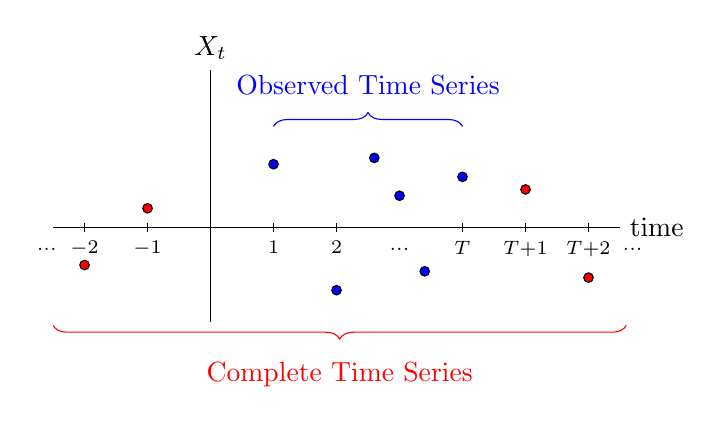
\begin{tikzpicture}[scale=0.8]
        \draw (-2.5,0) -- (6.5,0) node[right] {time};
        \draw (0,-1.5) -- (0,2.5) node[above] {$X_t$};

        \foreach \x/\xtext in {-2/-2, -1/-1, 1/1, 2/2, 4/T, 5/T+1, 6/T+2}
        \draw[shift={(\x,0)}] (0pt,2pt) -- (0pt,-2pt) node[below] {$\scriptstyle\xtext$};

        \draw (-2.6,0) node[below,yshift=-4pt] {$\scriptstyle\ldots$};
        \draw (3,0) node[below,yshift=-4pt] {$\scriptstyle\ldots$};
        \draw (6.7,0) node[below,yshift=-4pt] {$\scriptstyle\ldots$};

        \draw[fill=red] (-2,-.6) circle (.5ex);
        \draw[fill=red] (-1,0.3) circle (.5ex);
        \draw[fill=blue] (1,1) circle (.5ex);
        \draw[fill=blue] (2,-1) circle (.5ex);
        \draw[fill=blue] (2.6,1.1) circle (.5ex);
        \draw[fill=blue] (3,0.5) circle (.5ex);
        \draw[fill=blue] (3.4,-.7) circle (.5ex);
        \draw[fill=blue] (4,.8) circle (.5ex);
        \draw[fill=red] (5,.6) circle (.5ex);
        \draw[fill=red] (6,-.8) circle (.5ex);

        \draw [decorate,decoration={brace,amplitude=5pt,mirror,raise=4ex},color=red]
        (-2.5,-0.8) -- (6.6,-0.8) node[midway,yshift=-3.5em,text=red]{Complete Time Series};
        \draw [decorate,decoration={brace,amplitude=5pt},color=blue]
        (1,1.6) -- (4,1.6) node[midway,yshift=1.5em,text=blue]{Observed Time Series};
    \end{tikzpicture}
\end{figure}
The worst case: $ X_t\sim F_t $, where $ F_t $ is a \emph{changing}
function of $ t $. If so, it is hard to pool the data
$ X_1,\ldots,X_T $ to estimate $ F_t $. If
\textbf{serial dependence} occurs; that is, if the
distribution of $ (X_t,X_{t+h}) $
depends strongly on $ t $, then we have a similar problem in estimating
e.g., $ \Cov{X_t,X_{t+h}} $.

\begin{Definition}{Strictly stationary}{}
    We say that a time series $ \set{X_t}_{t\in\mathbf{Z}} $
    is \textbf{strictly stationary} (\textbf{strongly stationary})
    if for each $ k\ge 1 $, $ i_1,\ldots,i_k,h\in\mathbf{Z} $,
    \[ (X_{i_1},\ldots,X_{i_k})\stackrel{\text{d}}{=}
        (X_{i_{1}+h},\ldots,X_{i_k+h}) \]
    {\color{blue}If we look at the $ k $-dimensional joint distribution
    $ (X_{i_1},\ldots,X_{i_k}) $
    of the series at points $ i_1,\ldots,i_k $, then
    strict stationary means this is shift-invariant.}
    That is, shifting the window on which
    you view the data, does \underline{not} change its distribution.
    This implies that if $ F_t=\text{CDF} $ of $ X_t $, then
    $ F_t=F_{t+h}=F $; that is, all variables have a common distribution function.
\end{Definition}
\begin{Definition}{Mean function}{}
    For a time series $ \set{X_t}_{t\in\mathbf{Z}} $, with
    $ \E{X_t^2}<\infty $ for all $ t\in\mathbf{Z} $,
    we denote the \textbf{mean function} of the time series as
    \[ \mu_t=\E{X_t} \]
\end{Definition}
\begin{Definition}{Autocovariance function}{}
    The \textbf{autocovariance} function of the time series $ \set{X_t}_{t\in\mathbf{Z}} $
    is defined as
    \[ \gamma(t,s)=\E[\big]{(X_t-\mu_t)(X_s-\mu_s)}=\Cov{X_t,X_s} \]
\end{Definition}
\begin{Definition}{Weakly stationary, Lag}{}
    We say that a time series $ \set{X_t}_{t\in\mathbf{Z}} $
    is \textbf{weakly stationary} if $ \E{X_t}=\mu $
    which does not depend on $ t $, and if
    \[ \gamma(t,s)=f\bigl(\abs{t-s}\bigr) \]
    that is, $ \gamma(t,s) $ is a function of $ \abs{t-s} $. In this case,
    we usually write
    \[ \gamma(h)=\Cov{X_t,X_{t+h}} \]
    where we call the input $ h $ the \textbf{lag} parameter.
\end{Definition}
\subsection*{Additional Terminology}
\begin{itemize}
    \item The property when $ \E{X_t}=\mu $ which does not depend
          on $ t $ is often called \textbf{first order stationary}.
    \item The property when $ \gamma(t,s)=f\bigl(\abs{t-s}\bigr) $
          only depends on the lag $ \abs{t-s} $ is called
          \textbf{second order stationary}.
    \item For a second order stationary process,
          \begin{align*}
              \gamma(h)
               & =\Cov{X_t,X_{t+h}}                                      \\
               & =\Cov{X_{t-h},X_{t-h+h}} & \quad & t\rightarrow{} (t-h) \\
               & =\Cov{X_t,X_{t-h}}                                      \\
               & =\gamma(-h)
          \end{align*}
          Since $ \gamma(h)=\gamma(-h) $, we
          normally only record $ \gamma(h) $ for $ h\ge 1 $.
\end{itemize}
\section{White Noise and Stationary Examples}
\begin{Definition}{Strong white noise}{}
    We say $ \set{X_t}_{t\in\mathbf{Z}} $ is a
    \textbf{strong white noise} if $ \E{X_t}=0 $
    and the $ \set{X_t}_{t\in\mathbf{Z}} $ are i.i.d.
\end{Definition}
\begin{Definition}{Weak white noise}{}
    We say $ \set{X_t}_{t\in\mathbf{Z}} $ is a
    \textbf{weak white noise} if $ \E{X_t}=0 $
    and
    \[ \gamma(t,s)=\Cov{X_t,X_s}=\begin{cases}
            \sigma^2 & \abs{t-s}=0 \\
            0        & \abs{t-s}>0
        \end{cases} \]
\end{Definition}
\begin{Definition}{Gaussian white noise}{}
    We say $ \set{X_t}_{t\in\mathbf{Z}} $ is a
    \textbf{Gaussian white noise}
    if $ X_t\stackrel{\text{iid}}{\sim}\N{0,\sigma^2} $.
\end{Definition}
\begin{figure}[!htbp]
    \centering
    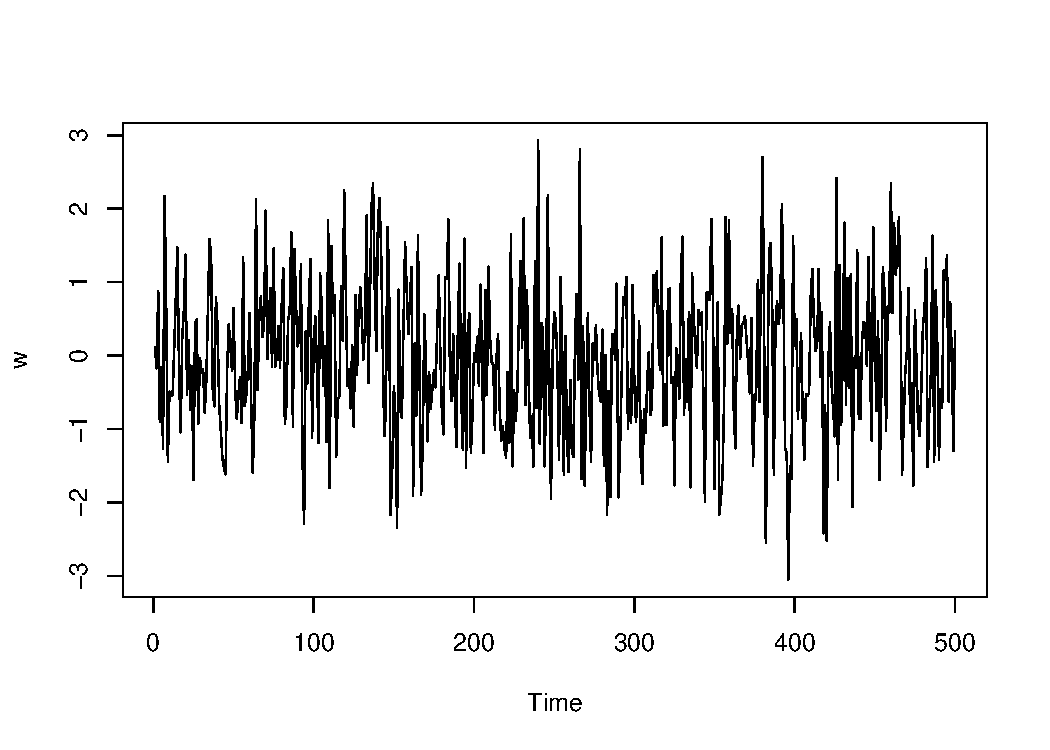
\includegraphics[width=0.75\textwidth]{wn.pdf}
    \caption{Gaussian White Noise of Length 500}\label{fig:wn}
\end{figure}
\begin{minted}{R}
# Figure 1.4
plot.ts(rnorm(500), main = "Gaussian White Noise", ylab = "w")
\end{minted}
Figure~\ref{fig:wn} is a Gaussian \emph{white} noise series.
\textbf{White} comes from spectral analysis,
in which a white noise series shares the same spectral properties as white light:
all periodicities occur with equal strength.
\begin{Example}{}{}
    Suppose $ \set{W_t}_{t\in\mathbf{Z}} $
    is a strong white noise, then $ \E{W_t}=0 $;
    that is, the mean of $ W_t $ doesn't depend on $ t $.
    \[ \gamma(t,s)=\Cov{W_t,W_s}=\E{W_t W_s}=
        \begin{cases}
            \sigma_W^2 & \abs{t-s}=0 \\
            0          & \abs{t-s}>0
        \end{cases} \]
    $ \gamma(t,s) $ only depends on $ \abs{t-s} $. Therefore,
    $ \set{W_t}_{t\in\mathbf{Z}} $ is
    \textbf{weakly stationary}. Furthermore,
    we claim that
    $ \set{W_t}_{t\in\mathbf{Z}} $ is
    \textbf{strictly stationary}. Let $ k\ge 1 $,
    $ i_1,\ldots,i_k,h\in\mathbf{Z} $ with $ i_1<\cdots<i_k $, then
    \begin{align*}
        \Prob{W_{i_1}\le t_1,\ldots,W_{i_k}\le t_k}
         & =\prod_{j=1}^k\Prob{W_{i_j}\le t_j}                   & \quad & \text{independence} \\
         & =\prod_{j=1}^k\Prob{W_{{i_j}+h}\le t_j}                                             \\
         & =\Prob{W_{{i_1}+h}\le t_1,\ldots, W_{{i_k}+h}\le t_k}
    \end{align*}
\end{Example}
\begin{Example}{}{}
    Suppose $ \set{W_t}_{t\in\mathbf{Z}} $ is a strong white noise.
    Define $ X_t=W_t+\theta W_{t-1} $ for $ \theta\in\mathbf{R} $.
    Since $ \set{W_t}_{t\in\mathbf{Z}} $ is a strong white noise, we
    have $ \E{W_t}=0 $ for all $ t $, hence we
    have $ \E{X_t}=\E{W_t+\theta W_{t-1}}=\E{W_t}+\theta\E{W_{t-1}}=0 $
    which is first order stationary.
    \[ \gamma(t,s)=\Cov{X_t,X_s}=\begin{cases}
            (1+\theta^2)\sigma_W^2 & \abs{t-s}=0 \\
            \theta\sigma_W^2       & \abs{t-s}=1 \\
            0                      & \abs{t-s}>0
        \end{cases} \]
    We obtain these calculations as follows:
    \begin{itemize}
        \item $ \abs{t-s}=0 $.
              \[ \E[\big]{(W_t+\theta W_{t-1})^2}
                  =\E{W_t^2}+\theta^2\E{W_{t-1}^2}+2\E{\theta W_t W_{t-1}}
                  =(1+\theta^2)\sigma_W^2 \]
              since $ W_t $ is independent of $ W_{t-1} $. The calculation is easy to verify.
        \item $ t=s+1 $ (or $ s=t+1 $).
              \[ \E[\big]{(W_{s+1}+\theta W_s)(W_s+\theta W_{s-1})}=\theta\E{W_s^2}=\theta\sigma_W^2 \]
              since $ W_{s+1} $ is independent of $ W_s $ and $ W_{s-1} $.
              The calculation is easy to verify.
        \item $ \abs{t-s}>1 $. $ W_t+\theta W_{t-1} $ is independent of
              $ W_s+\theta W_{s-1} $.
    \end{itemize}
    We claim that $ \set{X_t}_{t\in\mathbf{Z}} $ is also strictly stationary.
    Let $ k\ge 1 $, $ i_1,\ldots,i_k, h\in\mathbf{Z} $
    with $ i_1<\cdots<i_k $, then
    \begin{align*}
        \Prob{X_{i_1}\le t_1,\ldots,X_{i_k}\le t_k}
         & =\Prob{W_{i_1}+\theta W_{{i_1}-1}\le t_1,\ldots,W_{i_k}+\theta W_{{i_k}-1}\le t_k} \\
         & =\Prob*{\begin{bmatrix}
                W_{{i_1}-1} \\
                W_{i_1}     \\
                \vdots      \\
                W_{i_k}
            \end{bmatrix}\in \mathcal{B}}                                 \\
         & =\Prob*{\begin{bmatrix}
                W_{{i_1-1}+h} \\
                \vdots        \\
                W_{{i_k}+h}
            \end{bmatrix}\in \mathcal{B}}                                 \\
         & =\Prob{X_{{i_1}+h}\le t_1,\ldots,X_{{i_k}+h}\le t_k}
    \end{align*}
    where $ \mathcal{B} $ is some subset of $ \mathbf{R}^{i_k-i_1+1} $, and hence
    is shift-invariant.
\end{Example}
\begin{Definition}{Bernoulli shift}{}
    Suppose $ \set{\varepsilon_t}_{t\in\mathbf{Z}} $ is a
    strong white noise. If $ X_t=g(\varepsilon_t,\varepsilon_{t-1},\ldots) $
    for some function $ g:\mathbf{R}^\infty \to \mathbf{R} $, we say that
    $ \set{X_t}_{t\in\mathbf{Z}} $ is a \textbf{Bernoulli shift}.
\end{Definition}
\begin{Remark}{}{}
    We can also make a more general definition for a Bernoulli shift.
    Suppose $ \set{\varepsilon_t}_{t\in\mathbf{Z}} $ is a
    strong white noise. If $ X_t=g(\ldots,\varepsilon_{t-1},\varepsilon_t,\varepsilon_{t+1},\ldots) $
    for some function $ g:\mathbf{R}^\mathbf{Z} \to \mathbf{R} $, we say that
    $ \set{X_t}_{t\in\mathbf{Z}} $ is a \textbf{Bernoulli shift}.
\end{Remark}
\begin{Theorem}{}{}
    If $ \set{X_t}_{t\in\mathbf{Z}} $ is a Bernoulli shift, then
    $ \set{X_t}_{t\in\mathbf{Z}} $ is strictly stationary.
\end{Theorem}
\begin{Remark}{}{}
    Norbert Wiener conjectured that \textbf{every} stationary
    sequence is a Bernoulli shift, which is not true. The truth is,
    almost every one is.
\end{Remark}
\begin{Exercise}{}{}
    Suppose $ \set{W_t}_{t\in\mathbf{Z}} $ is a strong white noise.
    The \textbf{two-sided random walk} is defined as
    \[ X_t=\sum_{i=0}^{t} W_i+\sum_{i=t}^{-1} W_i  \]
    Show that $ \set{X_t}_{t\in\mathbf{Z}} $ is first order stationary,
    but $ \set{X_t}_{t\in\mathbf{Z}} $ is \underline{not} second order stationary.

    \textbf{Solution.} $ \set{X_t}_{t\in\mathbf{Z}} $ is first order stationary
    since
    \begin{align*}
        \E{X_t}
         & =\E[\bigg]{\sum_{i=0}^{t}W_i+\sum_{i=t}^{-1} W_i}                   \\
         & =\E{W_0+W_1+\cdots+W_{t-1}+W_{t}+W_{t}+W_{t-1}+\cdots+W_{0}+W_{-1}} \\
         & =\E{W_{-1}}+\E{2W_0}+\E{2W_1}+\cdots+\E{2W_{t-1}}                   \\
         & =0+2(0)+\cdots+2(0)                                                 \\
         & =0
    \end{align*}
    since $ \set{W_t}_{t\in\mathbf{Z}} $ is a strong white noise; that is,
    $ \E{W_t}=0 $ for all $ t $.

    $ \set{X_t}_{t\in\mathbf{Z}} $ is \underline{not} second order stationary
    since if $ t>0 $ the second sum is simply $ \sum_{i=t}^{-1} W_i=0 $, and we have
    \begin{align*}
        \E[\big]{(X_t-\mu_t)(X_t-\mu_t)}
         & =\E{X_t^2}                                                                                           \\
         & =\E*{\biggl(\sum_{i=0}^{t} W_i\biggr)^{\!2}}                                                         \\
         & =\E{W_0^2}+\cdots+\E{W_t^2}                  & \quad & \text{since $ W_i\indep W_j $ for $ i\ne j $} \\
         & =t\sigma_W^2
    \end{align*}
    which depends on $ t $.
\end{Exercise}
\section{Weak versus Strong Stationary}
Sadly, $ \set{X_t}_{t\in\mathbf{Z}} $ is strictly stationary does \underline{not} imply
$ \set{X_t}_{t\in\mathbf{Z}} $ is weakly stationary.
\begin{Example}{}{}
    Suppose $ X_t\stackrel{\text{iid}}{\sim} $ Cauchy Random Variables;
    that is,
    \[ \Prob{X_t\le s}=\int_{-\infty}^{s} \frac{1}{\pi(1+x^2)}\, d{x}  \]
    Then, $ \E{X_t} $ does not exist, and hence $ \set{X_t}_{t\in\mathbf{Z}} $ cannot
    be weakly stationary. However, $ \set{X_t}_{t\in\mathbf{Z}} $ is strictly
    stationary in this case since $ \set{X_t}_{t\in\mathbf{Z}} $ is a strong
    white noise.
\end{Example}
\begin{Theorem}{}{strongly_imp_weakly}
    If $ \set{X_t}_{t\in\mathbf{Z}} $ is strongly stationary and $ \E{X_0^2}<\infty $,
    then $ \set{X_t}_{t\in\mathbf{Z}} $ is weakly stationary.
\end{Theorem}
\begin{Proof}{\Cref{thm:strongly_imp_weakly}}{}
    Note that if $ \set{X_t}_{t\in\mathbf{Z}} $ is strictly stationary, then
    \[ (X_t)\stackrel{\text{d}}{=}(X_0) \]
    so that $ \E{X_t}=\E{X_0}=\mu $ which does not depend on $ t $, and also
    \[ \Var{X_t}=\Var{X_0} \]
    By the Cauchy-Schwarz inequality,
    \begin{align*}
        \gamma(t,s)
         & =\Cov{X_t,X_s}                                                                     \\
         & =\E[\big]{(X_s-\mu)(X_t-\mu)}                                                      \\
         & \le \set[\Big]{\E[\big]{(X_s-\mu)^2}}^{1/2}\set[\Big]{\E[\big]{(X_t-\mu)^2}}^{1/2} \\
         & =\sqrt{\Var{X_s}}\sqrt{\Var{X_t}}                                                  \\
         & =\Var{X_t}<\infty
    \end{align*}
    If $ t<s $, then
    \[ \Cov{X_t,X_s}=\Cov{X_0,X_{s-t}}=f\bigl(\abs{s-t}\bigr) \]
    since it is shift-invariant, and hence if we shift everything over by $ t $,
    \[ (X_t,X_s)\stackrel{\text{d}}{=}(X_{t-t},X_{s-t})\stackrel{\text{d}}{=}(X_0,X_{s-t}) \]
\end{Proof}
\begin{Definition}{Gaussian process}{}
    $ \set{X_t}_{t\in\mathbf{Z}} $ is said to be a
    \textbf{Gaussian process} (\textbf{Gaussian time series}) if
    for each $ k\in\mathbf{Z}_{\ge 1} $, $ i_1<i_2<\cdots<i_k $ we have
    \[ (X_{i_1},\ldots,X_{i_k})\sim
        \Mvn[\big]{\symbf{\mu}_k(i_1,\ldots,i_k),\Sigma_{k\times k}(i_1,\ldots,i_k)} \]
    \[ \symbf{\mu}_k=\begin{bmatrix}
            \E{X_{i_1}} \\
            \vdots      \\
            \E{X_{i_k}}
        \end{bmatrix}\quad
        \Sigma_{k\times k}=
        \Cov{X_{i_j},X_{i_r}}_{1\le j,\, r\le k} \]
\end{Definition}
\begin{Theorem}{}{weak_gaussian_imp_strictly}
    If $ \set{X_t}_{t\in\mathbf{Z}} $ is weakly stationary and is a Gaussian process, then
    $ \set{X_t}_{t\in\mathbf{Z}} $ is strictly stationary.
\end{Theorem}
\begin{Proof}{\Cref{thm:weak_gaussian_imp_strictly}}{}
    If $ \set{X_t}_{t\in\mathbf{Z}} $ is weakly stationary, then $ \E{X_t}=\mu $ for all $ t $.
    \[ (X_{i_1},\ldots,X_{i_k})\rightarrow
        \begin{bmatrix}
            \E{X_{i_1}} \\
            \vdots      \\
            \E{X_{i_k}}
        \end{bmatrix}=\begin{bmatrix}
            \mu    \\
            \vdots \\
            \mu
        \end{bmatrix}=\symbf{\mu}=
        \begin{bmatrix}
            \E{X_{{i_1}+h}} \\
            \vdots          \\
            \E{X_{{i_k}+h}}
        \end{bmatrix} \]
    Also,
    \begin{align*}
        \Var{X_{i_1},\ldots,X_{i_k}}
         & =\Cov{X_{i_j},X_{i_r}}_{1\le j,\, r\le k}       \\
         & =\Cov{X_0,X_{i_r-i_j}}_{1\le j,\, r\le k}       \\
         & =\Cov{X_0,X_{i_r+h-(i_j+h)}}_{1\le j,\, r\le k} \\
         & =\Cov{X_{i_j+h},X_{i_r+h}}_{1\le j,\, r\le k}   \\
         & =\Var{X_{i_1+h},\ldots,X_{i_k+h}}
    \end{align*}
    Using the Gaussian assumption
    \[ (X_{i_1},\ldots,X_{i_k})
        \stackrel{\text{d}}{=}\Mvn{\symbf{\mu},\symbf{\Sigma}_{k\times k}}
        \stackrel{\text{d}}{=}(X_{i_1+h},\ldots,X_{i_k+h}) \]
    Hence $ \set{X_{t}}_{t\in\mathbf{Z}} $ is strictly stationary
    in this case.
\end{Proof}
\begin{Exercise}{}{}
    Prove that if $ \set{X_t}_{t\in\mathbf{Z}} $ is \underline{not}
    weakly stationary; that is, either $ \E{X_t} $ depends on $ t $
    or $ \gamma(t,s) $ does not depend on the lag, and has
    a finite mean and variance,
    then $ \set{X_t}_{t\in\mathbf{Z}} $ is \underline{not} strictly stationary.
\end{Exercise}

\section{\texorpdfstring{$ \dagger $}{†} Theoretical L2 Framework for Time Series}
\begin{itemize}
    \item $ X_t = \lim\limits_{{h} \to {\infty}} X_{h,t} $. In what sense
          does this limit exist?
    \item How ``close'' are two random variables $ X $ and $ Y $?
    \item Is there a random variable that achieves
          \[ \inf_{y\in S}d(Y,S) \]
\end{itemize}
\begin{Definition}{$ L^2 $ space}{}
    Consider a probability space $ (\Omega,\mathcal{F},\mathbb{P}) $.
    The space $ L^2 $ is the set of random variables
    $ X:\Omega\to\mathbf{R} $ measurable so that $ \E{X^2}<\infty $.
\end{Definition}
\begin{Definition}{$ L^2 $-time series}{}
    We say that $ \set{X_t}_{t\in\mathbf{Z}} $ is
    and $ L^2 $-time series if $ X_t\in L^2 $ for all
    $ t\in\mathbf{Z} $.
\end{Definition}
$ L^2 $ is a Hilbert space when equipped
with inner product, $ X,Y\in L^2 $.
\[ \innerp{X}{Y}=\E{XY} \]
$ \innerp{}{} $ is an inner product since it is
\begin{enumerate}[(1)]
    \item Linear: $ \innerp{aX+bY}{Z}=a\innerp{X}{Z}+b\innerp{Y}{Z} $.
    \item ``Almost'' Positive Definite:
          $ \innerp{X}{X}=\E{X^2}=0 \iff X=0 $ almost surely; that is, $ \Prob{X=0}=1 $.
    \item Symmetric: $ \innerp{X}{Y}=\innerp{Y}{X} $.
\end{enumerate}
$ L^2 $ is complete with this inner product; that is,
whenever $ X_n\in L^2 $ so that $ \E[\big]{(X_n-X_m)^2}\to 0 $
as $ n,m\to\infty $, then there exists $ X\in L^2 $
so that $ X_n\to X $; that is, $ \E[\big]{(X_n-X)^2}\to 0 $.
This follows from the ``famous'' Riesz-Fischer Theorem.
\subsection*{Useful Tools for Time Series}
\begin{enumerate}[(1)]
    \item \textbf{Existence of Limits}
          \[ X_{t,n}=\sum_{j=0}^{n} \psi_j \varepsilon_{t-j}
          \]
          $ \set{\varepsilon_t}_{t\in\mathbf{Z}} $ is a strong white noise.
          Since for $ n>m $,
          \[ \E[\big]{(X_{t,n}-X_{t,m})^2}
              =\E*{\biggl(\sum_{j=m+1}^{n} \psi_j \varepsilon_{t-j}\biggr)^{\!2}}
              =\sum_{j=m+1}^{n} \psi_j^2\sigma_{\varepsilon}^2\to 0\text{ as }
              n,m\to \infty \]
          only if $ \sum_{j=0}^{\infty} \psi_j^2<\infty $, then there \textbf{must}
          exist a random variable $ X_t $ (by the completeness of $ L^2 $), so that
          \[ X_t=\lim\limits_{{n} \to {\infty}} X_{t,n}=\sum_{j=0}^{\infty}
              \psi_j \varepsilon_{t-j} \]
    \item \textbf{Projection Theorem and Forecasting}.
          Forecasting can be often cast as finding a random variable $ Y $ among
          a collection of possible forecasts $ \mathcal{M} $ (e.g.,
          $ \mathcal{M}=\Span{X_T,\ldots,X_1} $) so that
          \[ Y=\arginf_{Z\in\mathcal{M}}\E[\big]{(X_{T+h}-Z)^2} \]
          When $ \mathcal{M} $ is a closed linear subspace of $ L^2 $,
          the Projection Theorem guarantees that such a $ Y $ exists,
          and it must satisfy
          \[ \innerp{X_{T+h}-Y}{Z}=0\quad\forall Z\in\mathcal{M} \]
          must be in the orthogonal complement.
\end{enumerate}

\section{Signal and Noise Models}
``Ideally,'' a time series that we are considering
was generated from a stationary process. If so,
we can pool data to estimate the processes underlying structure
(e.g., its marginal distribution, and serial dependence structure).

Most time series are evidently \underline{not} stationary.

Looking back at Figure~\ref{fig:jj}:
\begin{itemize}
    \item Mean appears to increase, so it is not first order stationary;
    \item Variability also appears to increase, so it is not
          second order stationary;
    \item Therefore, it is not strictly stationary.
\end{itemize}
Signal and Noise Model: $ X_t=s_t+\varepsilon_t $
\begin{itemize}
    \item $ s_t $ is the \textbf{deterministic}
          ``signal'' or ``trend'' of the series.
    \item $ \varepsilon_t $ is the ``noise'' added
          to the signal satisfying $ \E{\varepsilon_t}=0 $, hence
          $ \E{X_t}=\E{s_t+\varepsilon_t}=\E{s_t} $.
          There exists a (strong) white noise $ \set{W_t}_{t\in\mathbf{Z}} $
          so that
          \[ \varepsilon_t=g(W_t,W_{t-1},\ldots)\quad\text{[Stationary Noise]} \]
          \[ \varepsilon_t=g_t(W_t,W_{t-1},\ldots)\quad\text{[Non-stationary Noise]} \]
          The terms $ \set{W_t}_{t\in\mathbf{Z}} $ are often called the
          ``innovations'' or ``shocks'' driving the random behaviour
          of $ X_t $.

              {\color{blue}$ g $ is used to try to capture noise that can
                  potentially have serial dependence.}
\end{itemize}
\begin{Example}{}{}
    An example of a function $ g $ so that $ \varepsilon_t=g_t(W_t,W_{t-1},\ldots) $
    might be a \textbf{random walk}; that is, $ \varepsilon_t=\sum_{j=0}^{t} W_j $.
    Another example could be the \textbf{changing variance models}; that is,
    $ \varepsilon_t=\sigma(t)W_t $.
\end{Example}
Our goal is to estimate $ s_t $, and then infer the structure of $ \varepsilon_t $.

In Figure~\ref{fig:gtemp}, the model appears to be non-stationary
(trending upwards over time),
so we might try the signal and noise model. We might posit
a linear trend, or even higher order functions.

For the temperature data, we may posit that
\[ s_t=\beta_0+\beta_1 t\quad\text{[Linear Trend]} \]
The trend may be estimated by ordinary least squares (OLS).
We choose $ \beta_0 $ and $ \beta_1 $ to minimize
\[ \sum_{t=1}^{T} \bigl[X_t-(\beta_0+\beta_1 t)\bigr]^2 \]
This can be done in R using the \code{lm()} command, and
can easily be computed with calculus. Figure~\ref{fig:gtemp_lm}
is a small example of the global temperature data superimposed
with the \code{lm()} estimate.
\begin{figure}[!htbp]
    \centering
    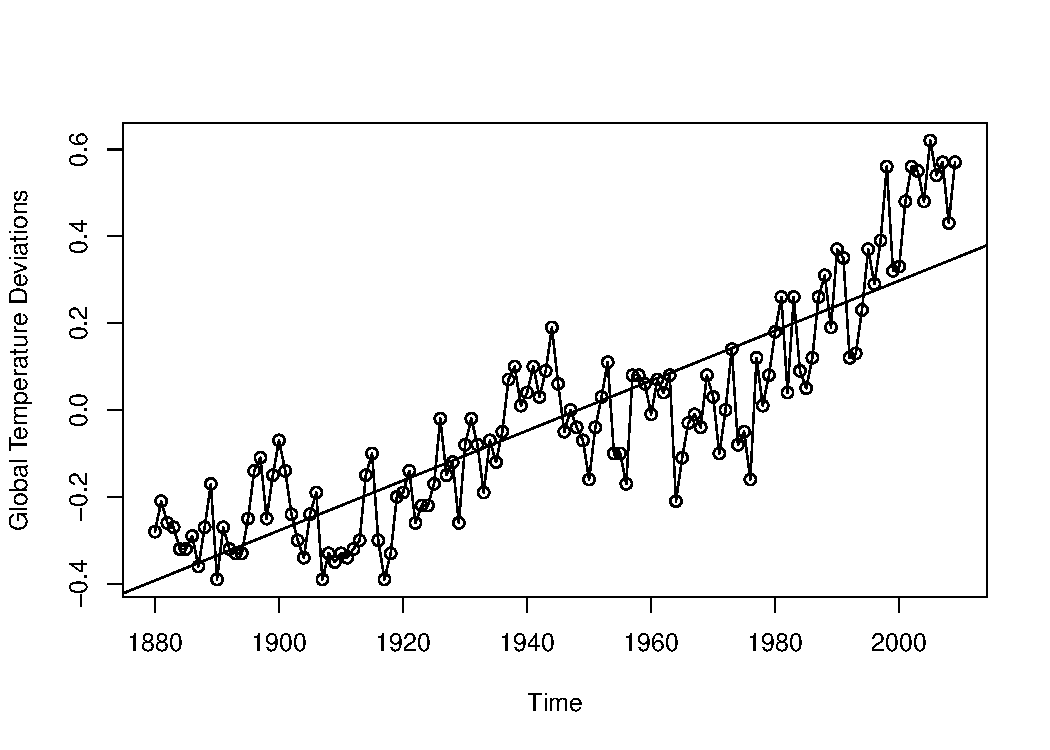
\includegraphics[width=0.75\textwidth]{gtemp_lm.pdf}
    \caption{OLS estimate of linear trend}\label{fig:gtemp_lm}
\end{figure}
\begin{minted}{R}
# Figure 1.5
fit <- lm(gtemp ~ time(gtemp), na.action = NULL)
plot.ts(gtemp, type = "o", ylab = "Global Temperature Deviations")
abline(fit)
\end{minted}
Let's introduce some terminology about trends.
\begin{Definition}{Detrended time series}{}
    Detrending a time series constitutes computing the
    residuals based on an estimate for the signal/trend.

    A \textbf{detrended time series} is a time series of such residuals.
    \begin{enumerate}
        \item Estimate $ s_t\to \hat{s_t} $.
        \item Detrend series: $ X_t-\hat{s_t}=Y_t $
              where $ Y_t $ is the ``detrended'' series.
    \end{enumerate}
\end{Definition}
\begin{figure}[!htbp]
    \centering
    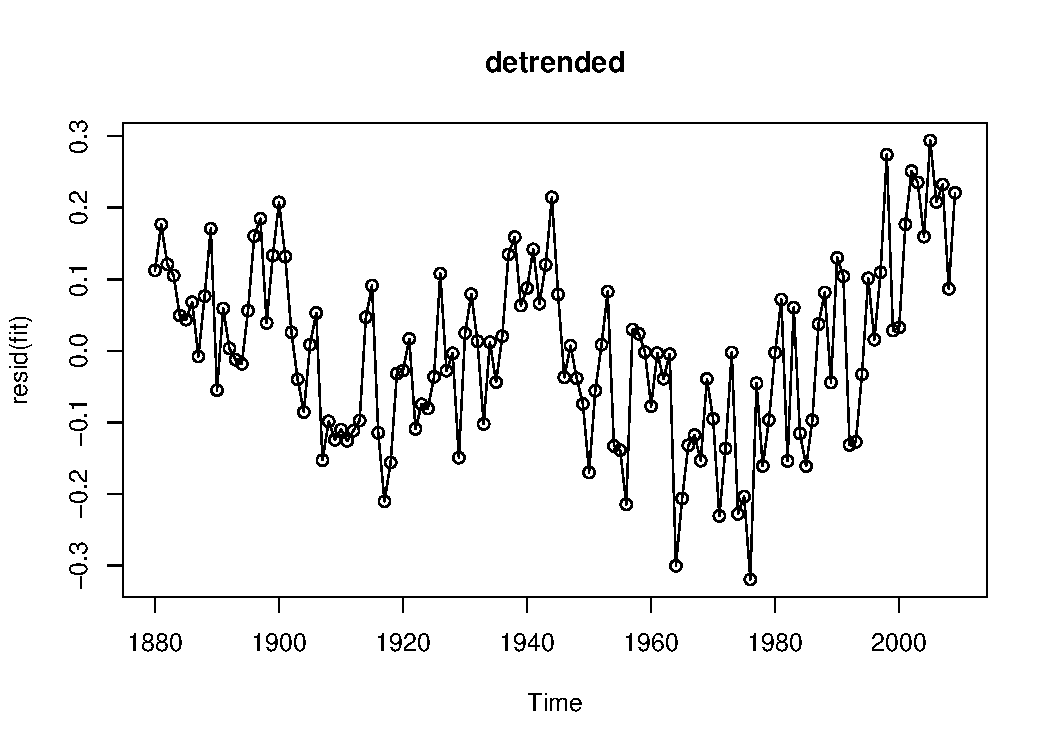
\includegraphics[width=0.75\textwidth]{detrended.pdf}
    \caption{Residuals of OLS fit.}\label{fig:detrended}
\end{figure}
\begin{minted}{R}
# Figure 1.6
plot(resid(fit), type = "o", main = "detrended")
\end{minted}
In Figure~\ref{fig:detrended}:
If trend is now zero, there appears to be a substantial serial
dependence remaining in the time series.

\section{Time Series Differencing}
Signal and Noise Model: $ X_t=s_t+\varepsilon_t $. Hopefully,
upon estimating $ s_t $ with $ \hat{s}_t $,
we find $ X_t-\hat{s}_t=\hat{\varepsilon}_t $ (detrended series)
which looks reasonably stationary. If the residuals were
reasonably stationary, we might
proceed in estimating their underlying structure of $ \set{\hat{\varepsilon}_t}_{t=1,\ldots,T} $
as if it were stationary. {\color{blue}In particular, we might try to estimate their marginal
        distributions and/or their serial dependence structure. If we thought those estimates
        were reasonably good, we would have a good idea of how the time series $ X_t $ behaves.}

\textbf{Random Walk with Drift Model}. Let $ \varepsilon_t $ be a strong white noise.
\begin{align*}
    X_t
     & =\delta+X_{t-1}+\varepsilon_t                                                                                  \\
     & =\delta+\delta+X_{t-2}+\varepsilon_{t-1}+\varepsilon_t                                                         \\
     & =\delta+\delta+\delta+X_{t-3}+\varepsilon_{t-2}+\varepsilon_{t-1}+\varepsilon_{t}                              \\
     & \vdots                                                                            & \quad & \text{$ t $ times} \\
     & =t\delta+X_0+\sum_{j=1}^{t} \varepsilon_j
\end{align*}
where we note that $ t\delta+X_0=s_t $ is a linear signal,
and $ \sum_{j=1}^{t} \varepsilon_j $ is a
random walk noise.

Notice that under the Random Walk Model.
\[ X_t-X_{t-1}=\nabla X_t=\delta+\varepsilon_t \]
So, if $ X_t $ follows a random walk model, the series $ Y_t=\nabla X_t $
should behave like a white noise shifted by $ \delta $.
\begin{figure}[!htbp]
    \centering
    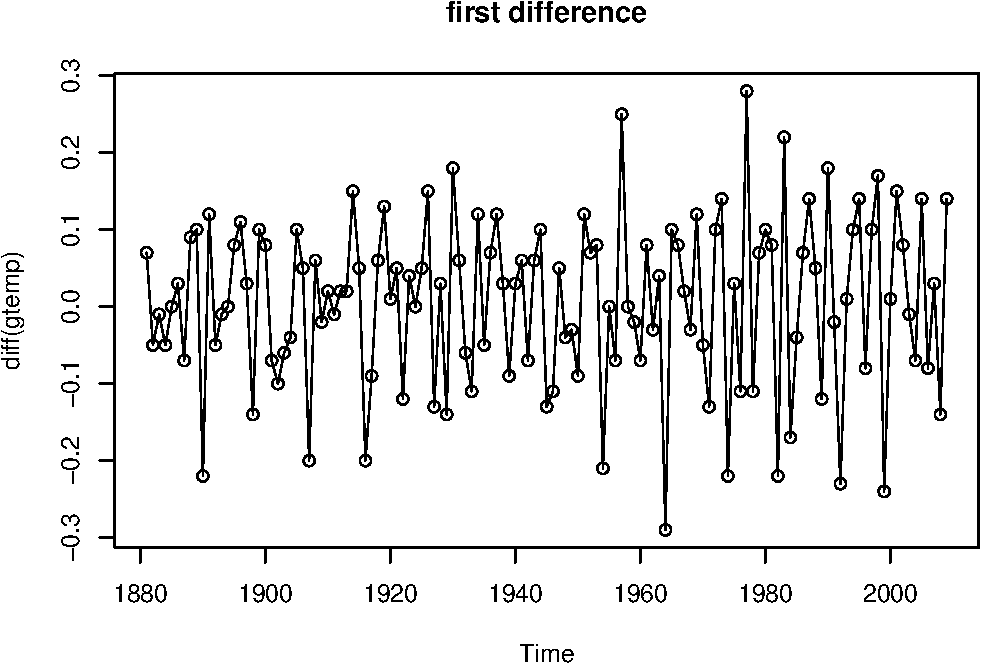
\includegraphics[width=0.75\textwidth]{first-diff.pdf}
    \caption{First differenced series. Average of first differenced series
        is $ \hat{\delta}\approx 0.0066 $}\label{fig:firstdiff}
\end{figure}
\begin{minted}{R}
# Figure 1.7
plot(diff(gtemp), type = "o", main = "first difference")
\end{minted}
In Figure~\ref{fig:firstdiff}:
{\color{blue}To see what this looks like in this temperature example, here is a plot
of $ \nabla X_t=X_t-X_{t-1} $ for~\Cref{fig:gtemp}. As you can
see if you look at this compared to the detrended series using linear trend,
I would say this series looks much more like a white noise (there does not
appear to be any discernible patterns in this first difference). If you calculate the mean
of this first difference series, that would be an estimator for the drift term
in the random walk model which here is $ \approx 0.0066 $.}

\begin{Definition}{Differenced time series}{}
    Differencing a time series constitutes
    computing the difference between successive terms.

    A \textbf{differenced time series} is a time series of such differences.
    The first differenced series is denoted
    \[ \nabla X_t=X_t-X_{t-1} \]
    and is the series of length $ T-1 $, namely
    \[ X_2-X_1,X_3-X_2,\ldots,X_T-X_{T-1} \]
    Higher order differences are calculated recursively, so
    \[ \nabla^d X_t=\nabla^{d-1}\nabla X_t \]
    where $ \nabla^d $ is the $ d^{\text{th}} $ order difference, and
    we define $ \nabla^0 X_t=X_t $.
\end{Definition}

Detrending and Differencing are both ways of reducing a
(potentially non-stationary) time series
to an approximately stationary series.

\subsection*{Differencing vs. Detrending}
\textbf{Pros}:
\begin{itemize}
    \item Differencing does not require the parameter estimation
          (don't need to estimate $ s_t $).
    \item Higher order differencing can reduce even very
          ``trendy'' series to look more like noise.
\end{itemize}
\textbf{Cons}:
\begin{itemize}
    \item Differencing can ``wash away'' features of the series,
          and introduce more complicated structures.
    \item The trend is often of interest, and good estimates
          of the trend lead to improved long-range forecasts.
\end{itemize}
\begin{Example}{Potentially Complicating Series with Differencing}{}
    $ X_t=W_t $ where $ W_t $ is a strong white noise.
    \[ \nabla X_t=W_t-W_{t-1}=Y_t \]
    \[ \gamma_X(h)=\Cov{X_t,X_{t+h}}=\begin{cases}
            \sigma_W^2 & h=0    \\
            0          & h\ge 1
        \end{cases} \]
    More complicated:
    \[ \gamma_Y(h)=\Cov{Y_t,Y_{t+h}}=\begin{cases}
            2\sigma_W^2 & h=0    \\
            -\sigma_W^2 & h=1    \\
            0           & h\ge 2
        \end{cases} \]
\end{Example}
\begin{figure}[!htbp]
    \centering
    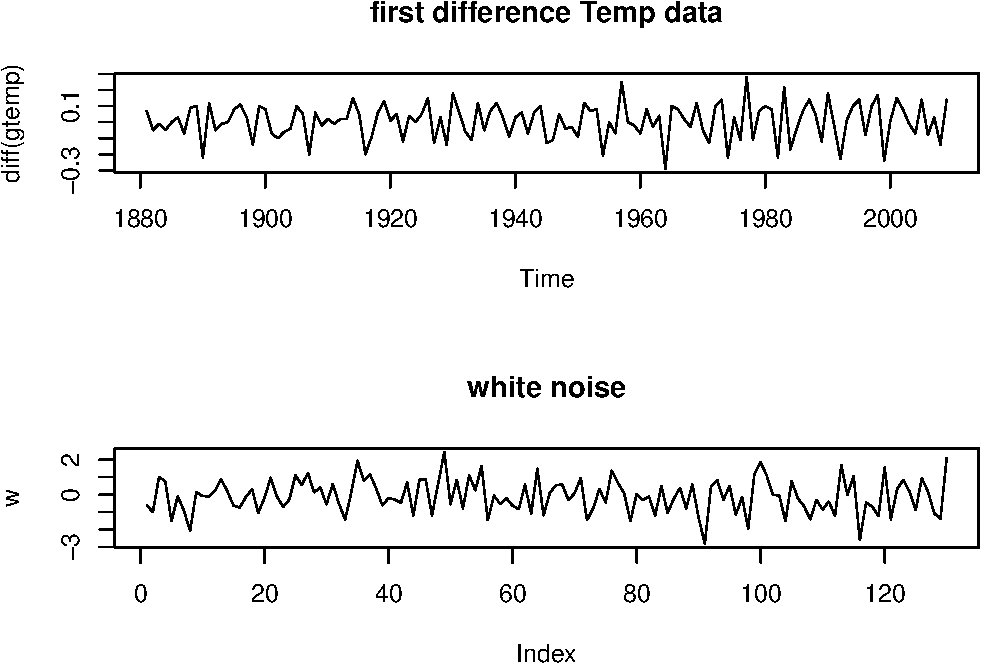
\includegraphics[width=0.75\textwidth]{firstdiffwn.pdf}
    \caption{First Difference and White Noise}\label{fig:firstdiffwn}
\end{figure}
\begin{minted}{R}
# Figure 1.8
par(mfrow = c(2, 1))
plot(diff(gtemp), main = "first difference Temp data")
plot(rnorm(gtemp),
     type = "l",
     main = "white noise",
     ylab = "w")    
\end{minted}
In Figure~\ref{fig:firstdiffwn}: If these two series behave in
the same way, then it stands to reason that
\[ g(\varepsilon_t,\varepsilon_{t-1},\ldots)=\varepsilon_t
    \stackrel{\text{iid}}{\sim}\N{0,\sigma^2_{\text{temp}}} \]
